\documentclass{uwmslide}
\usepackage{graphicx}
\usepackage{colordvi}
\title{{\tt uwmslide.cls} Test \& Example File}
\author{E. L. Benedict \\University of Wisconsin--Madison}
\date{26 September 2000}
\begin{document}
\textBlack
\maketitle


\begin{itemslide}{Outline}
\item The {\tt uwmslide} Class
\item The {\tt uwmslide} Class's Environments
\begin{itemize}
\item {\tt  slide}
\item {\tt  itemslide}
\item {\tt  doubleslide}
\item {\tt  leftitem}
\item {\tt  rightitem}
\item {\tt  doubleitem}
\end{itemize}
\item Color Example
\item Electronic Presentation
\item Conclusions
\end{itemslide}

\begin{slide}{The {\tt uwmslide} Class}
This \LaTeXe{} class allows for the easy production of slide presentations.
It is based on the {\tt article} class and provides several default slide
configurations.

This class automatically selects the PS Times font family for compatibility
with Adobe Acrobat files as well as setting the default to be landscape.
The required Postscript specials have been included to configure {\tt dvips}
to produce the properly rotated output by default.  This class also provides
the ability to include a logo file ({\tt logo.eps}) in the upper left corner.  
If the logo file is not present, it is omitted with a warning.

Several different slide environments are provided.  This slide was produced
using the plain {\tt slide} environment.
\end{slide}

\begin{itemslide}{The Item Slide}
\item Used to generate a slide which has bulleted Items.
\item The slide consists of a standard {\tt itemize} environment.
\item[$\spadesuit$] Bullets can be changed as usual.
\begin{itemize}
\item Sub items are possible
\item which would be expected
\end{itemize}
\end{itemslide}

\begin{doubleslide}{The Double Slide}
The double slide creates two minipages which allows you to put two columns in the
slide.  Here, there are text and equations on the left and a picture on the right.

\[V_{\rm aux}^{\rm max}=\sqrt{0.5 - 0.5\cos\left(2\tan^{-1}(\alpha)\right)}\]

$\alpha=$Auxilliary:Main Turns Ratio
\slidedivider
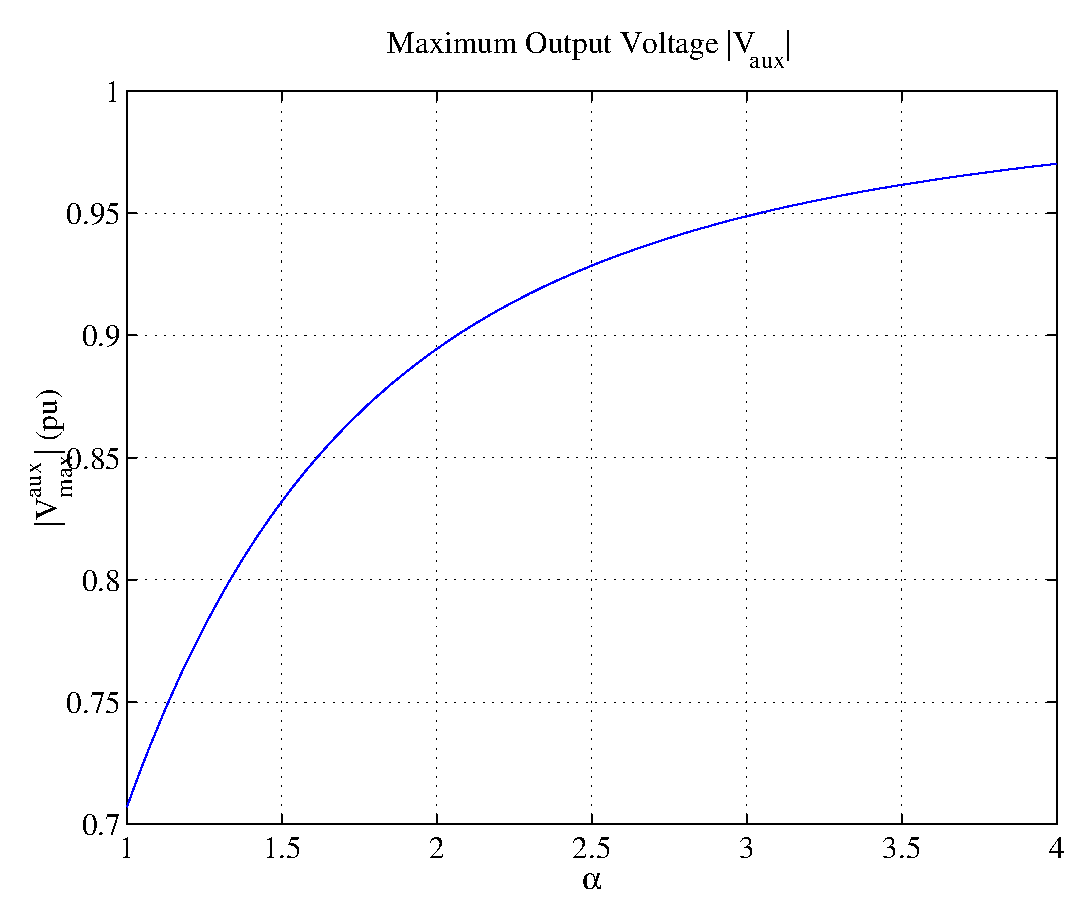
\includegraphics[width=4in]{vaux.eps}
\end{doubleslide}

\begin{leftitem}{The Left Item Slide}
\item Creates an Itemized List on the left
\item Creates a Minipage on the right
\item Great for figures and bullet lists
\slidedivider
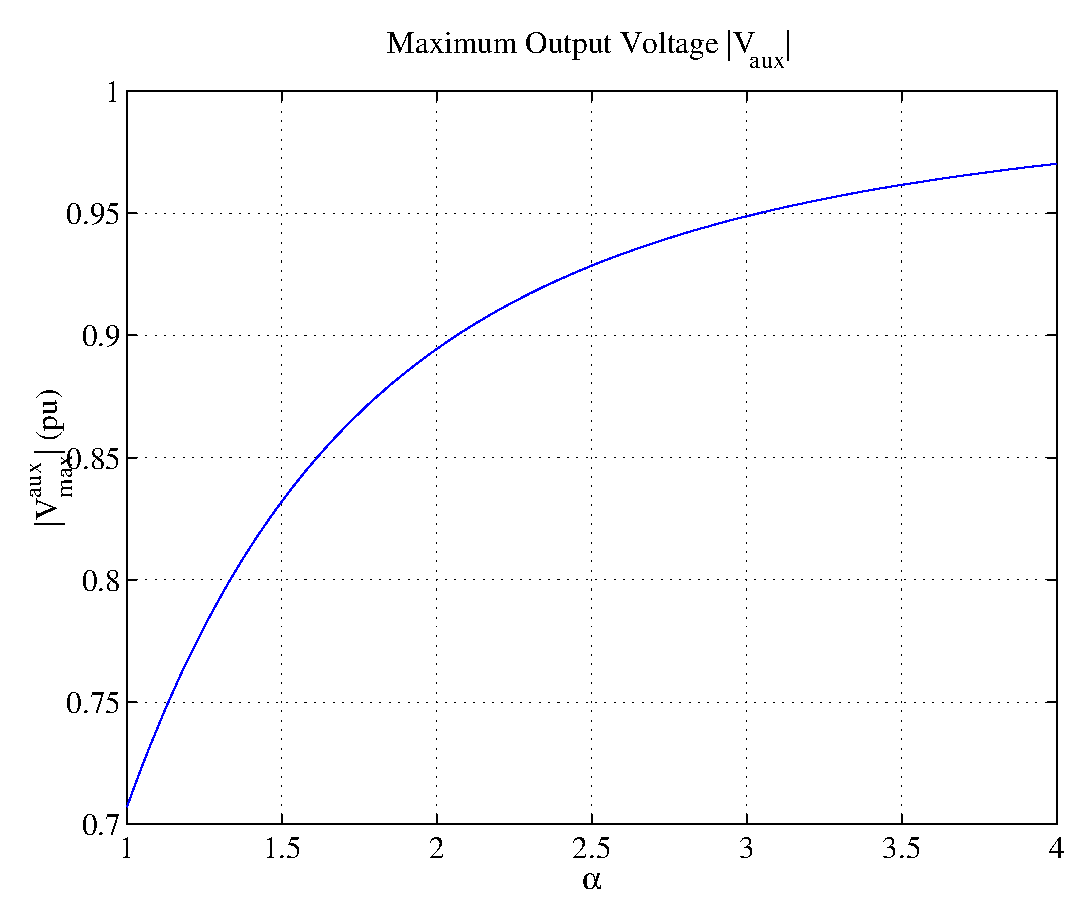
\includegraphics[width=4in]{vaux.eps}
\end{leftitem}


\begin{rightitem}{The Right Item Slide}
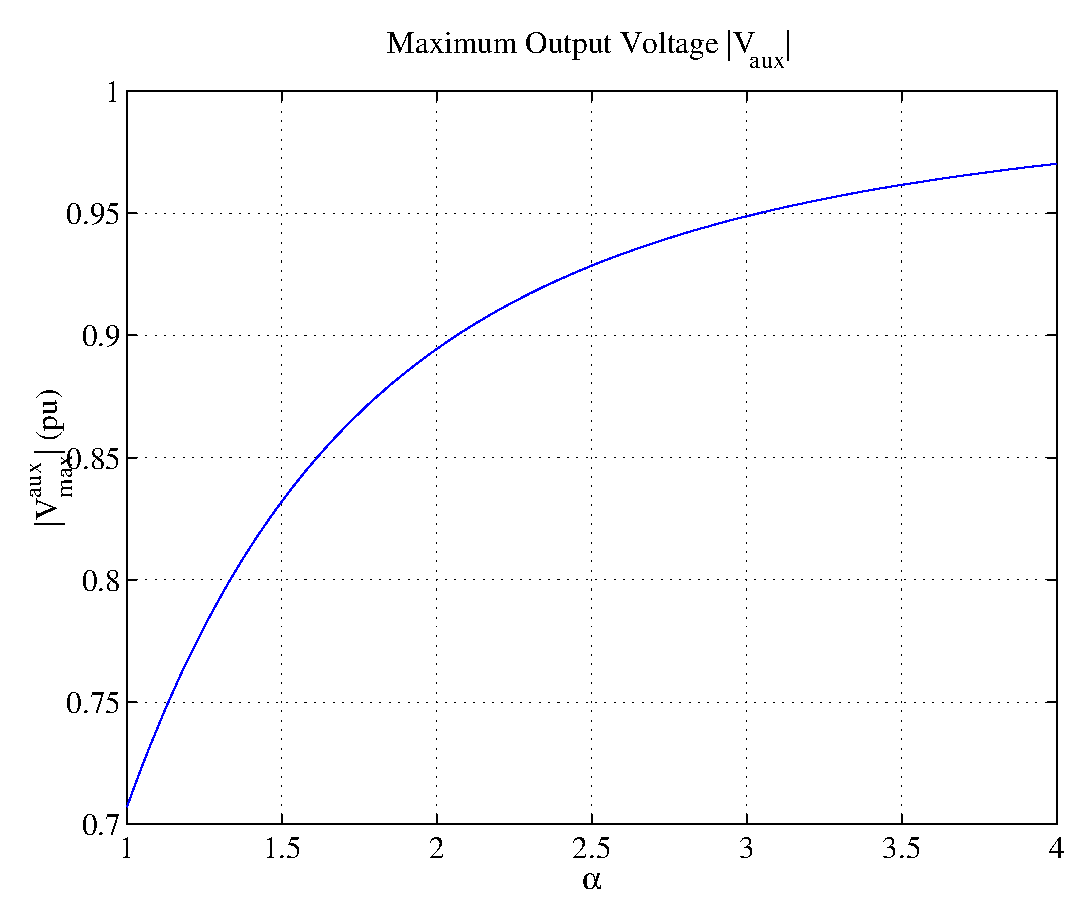
\includegraphics[width=4in]{vaux.eps}
\slidedivider
\item Creates an Itemized List on the Right
\item Creates a Minipage on the Left
\item Great for figures and bullet lists
\end{rightitem}

\begin{doubleitem}{The Double Item Slide}
\item  An Itemized List on the Left
\item Another Comment
\item A further Comment
\slidedivider
\item And an Itemized List on the Right
\item Another Comment
\item A further Comment
\end{doubleitem}

\begin{leftitem}[6.25in]{Variable Column Sizes}
\item  The column sizes for 
\begin{itemize}
\item \verb+ doubleslide+
\item \verb+ leftitem+
\item \verb+ rightitem+
\item \verb+ doubleitem+
\end{itemize}
are adjustable
\item This is 6.25" instead of the default 4.25"
\item Good for words like {\em antidisestablishmentarianism.}
\slidedivider
 Just include the optional argument of
the width of the left column to adjust the
column sizes.
\end{leftitem}

\begin{itemslide}{ \Red{Color} Slides}
\item Compatible with the package {\tt colordvi}
\item \Green{So you can specify different colors}
\item [$\spadesuit$] \Blue{Bullets can be changed as usual.}
\item You can \Magenta{emphasize} single words.
\item The color names come from the Crayola crayon box
\item[\Black{$\bullet$}] \Cyan{Cyan} \Brown{Brown} \Yellow{Yellow}
\Violet{Violet} \Purple{Purple} \Maroon{Maroon} 
\end{itemslide}

\begin{itemslide}{Conclusions}
\item The {\tt uwmslide} class allows the easy production of presentation slides
\item If the Postscript file is converted to an Adobe Acrobat format file, then
the Acrobat Reader program can be used to present the slides electronically. 
(Select the {\em Full Screen} option)
\item The logo file {\tt logo.eps} will be included for each slide, so try to
keep the logo file small, otherwise for larger presentations, the resulting file
will be excessively large.
\item Since the logo and the fonts all require Postscript, viewing the {\tt
*.dvi} file will produce non-representative results!
\end{itemslide}
\end{document}
